\subsection{Overview} 
Here we provide a high level representation of client-server interaction.
The client sends a request to the orchestrator who dispatches the request to the appropriate component. Both, components and orchestrator, are stateless. We thought to use the elastic component architectural pattern for the components. Moreover the orchestrator can eventually be duplicated using a fixed dimension  pool whoseconfigurable by the system administrator.

	\begin{figure}[H]	
	\centerline{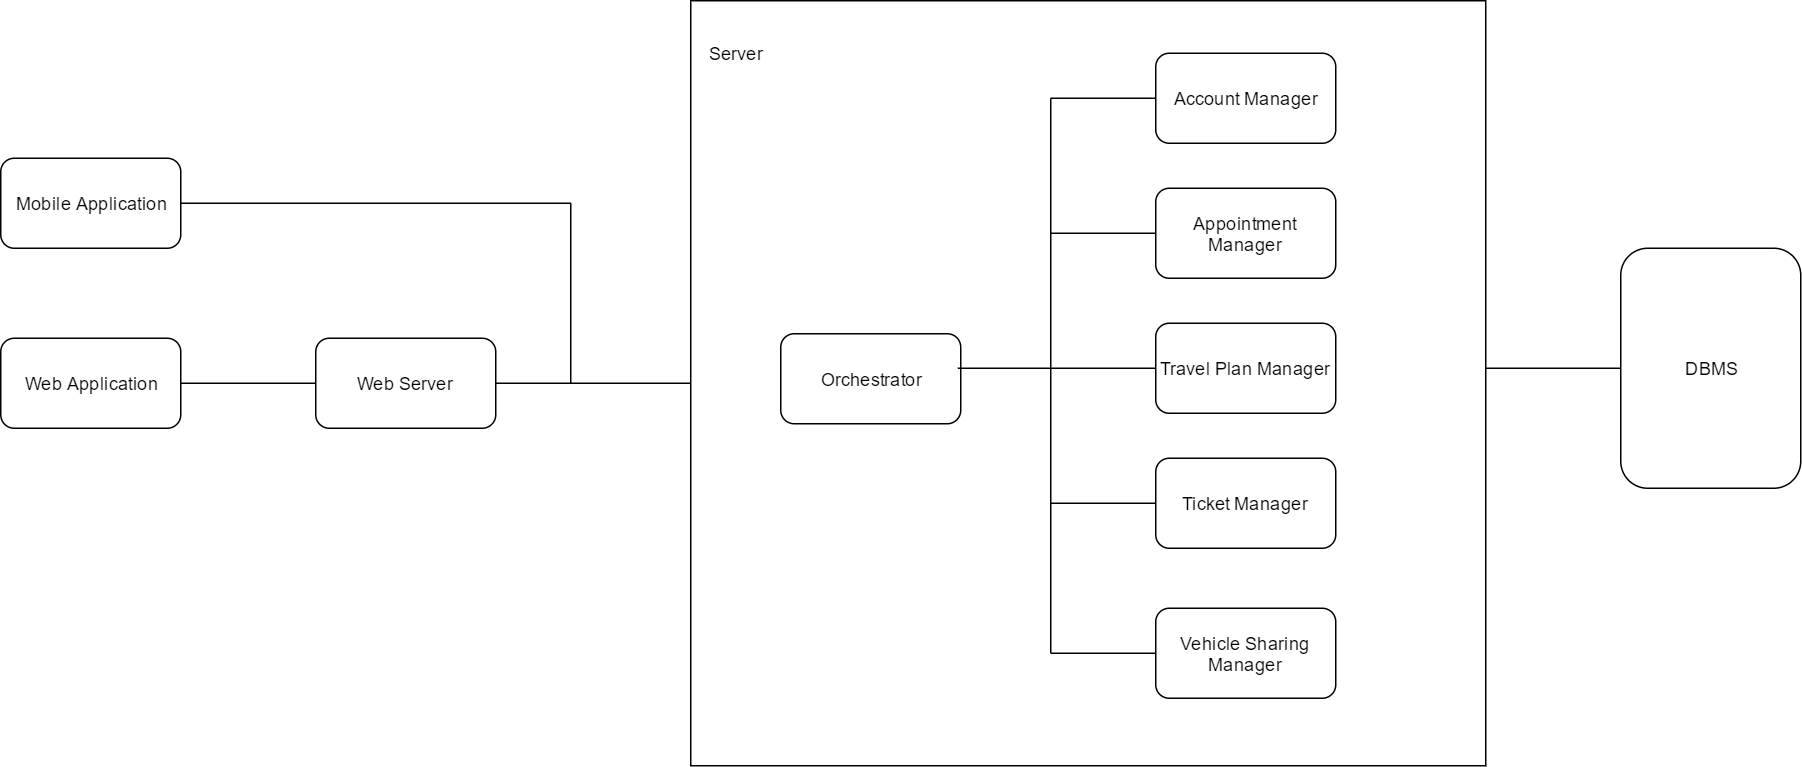
\includegraphics[width=0.9\paperwidth]{Images/HighLevelArchitecture}}
	\caption{High level Architecture Diagram - Client-Server interaction}
	\end{figure}	
\subsection{Component view}
	In the following diagrams we include a fictitious component, App, that will be highlighted in green and serves the purpose of representing both the mobile app and the web app (through the web server), without adding complexity to the diagrams.
	\subsubsection{Appointment Manager and Notification Manager}
		\label{sect:AppointmentManager}
		\label{sect:NotificationManager}
		Here we define the Appointment Manager and the Notification Manager. The Notification Manager will appear in others diagrams, but only here is detailed with its subcomponents. 
		\medskip\newline
		Appointment Manager has three subcomponents:		
		\begin{description}[before={\renewcommand{\makelabel}[1]{-- \textit{##1}:}}]
			\item[Appointment Handler] it is the only subcomponents communicating with the database: it manages all the read and write operations related to appointments. It is responsible for the final consistency check of the appointment before writing it to database. It exports an interface to external components to read appointments details and an internal interface to let subcomponents of Appointment Manager read and write appointments' details.
			\item[Appointment Editor] this provides an interface to easily change appointments' details and store it to database through the interface of Appointment Handler. Every time an appointment is created or details of an appointment changes, this send to Incoming Appointment Scheduler the appointment. This module interacts with an external module "Solution Calculator" to compute travel solutions. In this diagram it is displayed in dashed line because it will be described in another diagram.
			\item[Incoming Appointment Scheduler] for each appointment (provided by Appointment Editor) this module executes an algorithm to decide when that specific appointment will become an \defined{incoming appointment}. An appointment becomes incoming according to a combination of the time of the appointment and the travel plan chosen, to let the User receive a notification at an appropriate time. This is done generating a \defined{future notification} through the interface provided by Notification Manager.
		\end{description}
		\bigskip
		Notification Manager provide an interface for the creation of new notification and it is composed by two module:
		\begin{description}[before={\renewcommand{\makelabel}[1]{-- \textit{##1}:}}]
			\item[Notification Scheduler] this is the module whose interface is actually exported and it manages the creation of new notifications, stores them in the database and schedules their dispatch. When it is time to send a notification this module uses the interface provided by Notifier and delegate to it the dispatching procedure.
			\item[Notifier] it is in charge of the actual dispatch of the notification.
		\end{description}
		
		\begin{figure}[H]	
			\centerline{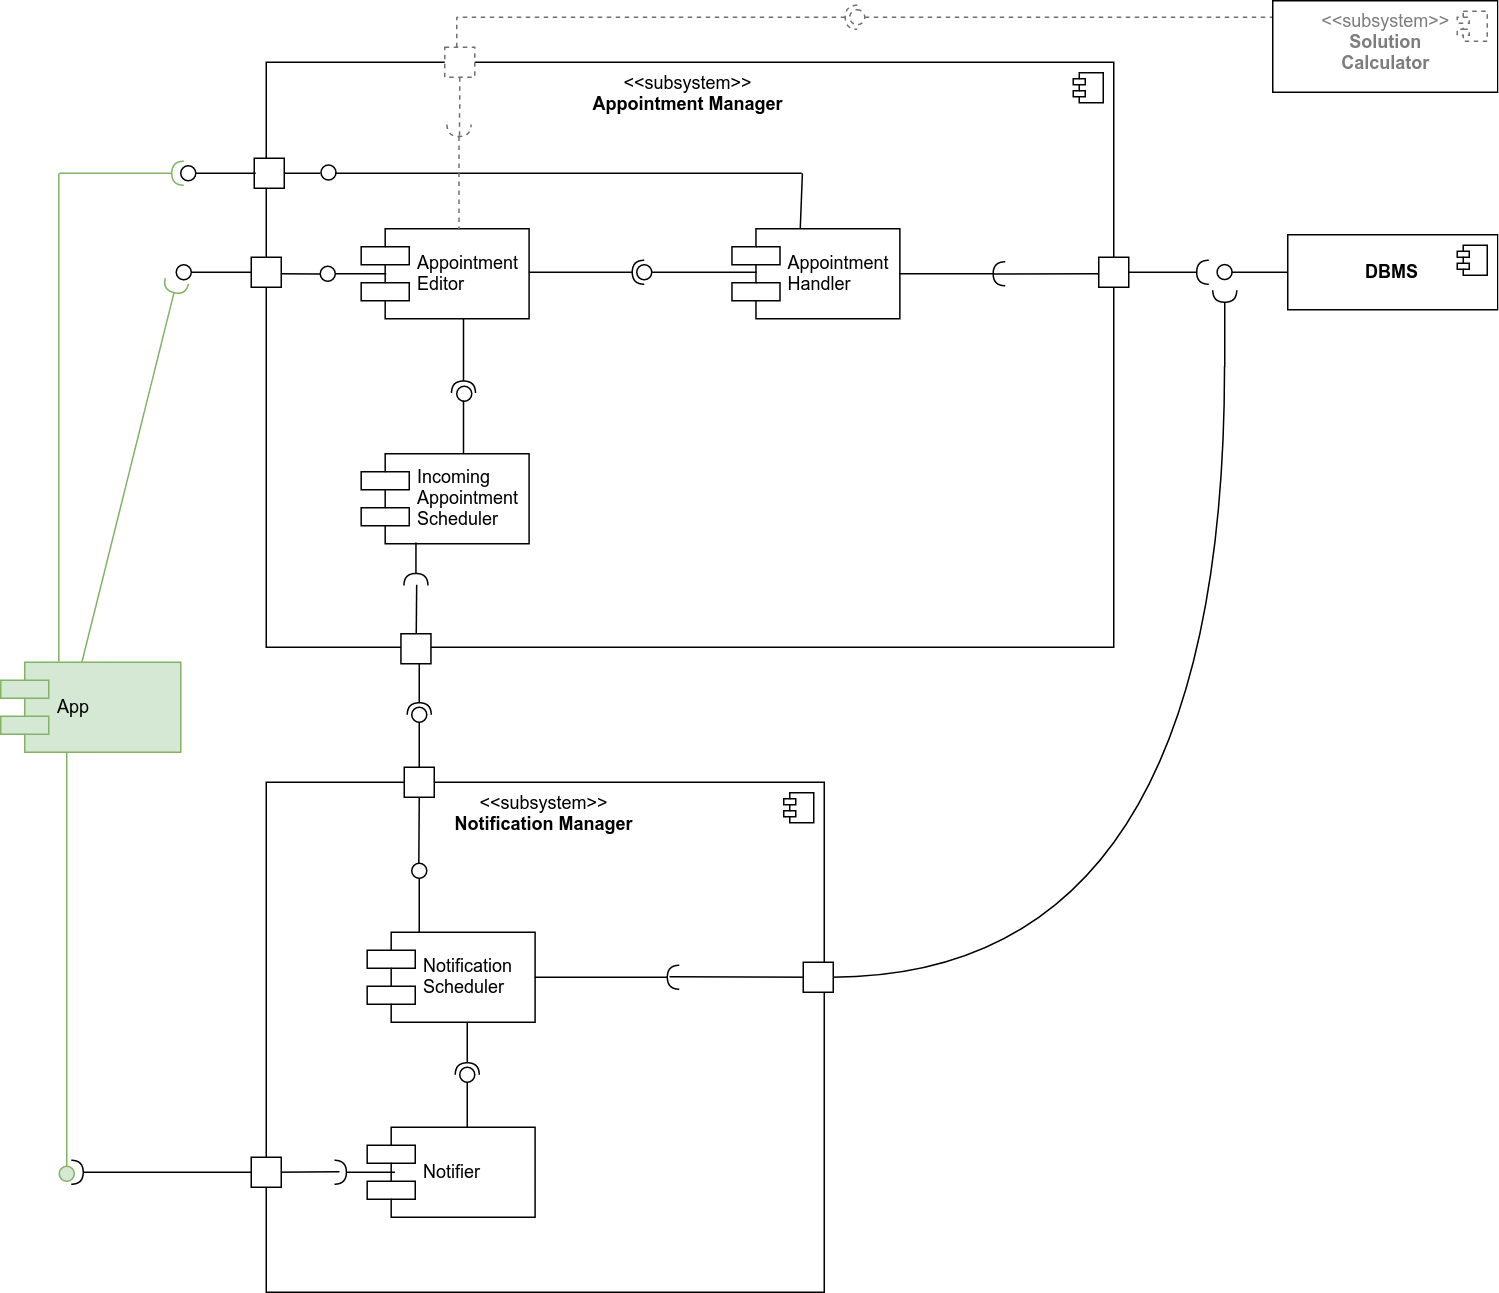
\includegraphics[width=0.9\paperwidth]{Images/CD_AppointmentManager}}
			\caption{Component Diagram - Appointment Manager \& Notification Manager}
		\end{figure}
		
	\subsubsection{Invitation Manager}
		\label{sect:InvitationManager}
		The Invitation Manager component is the module that manages all the aspects related to invitations, from their creation to the acceptance/refusal of the invited Users/Persons. It is divided into two subcomponents. A sequence diagram is provided in section \ref{sect:RuntimeView}.
		\begin{description}[before={\renewcommand{\makelabel}[1]{-- \textit{##1}:}}]
			\item[Invitation Generator] it manages the creation of a new invitations 
			\item[Invitation Handler] it is concerned with the acceptance/refusal of the invitations sent.
		\end{description}
		
		\begin{figure}[H]	
			\centerline{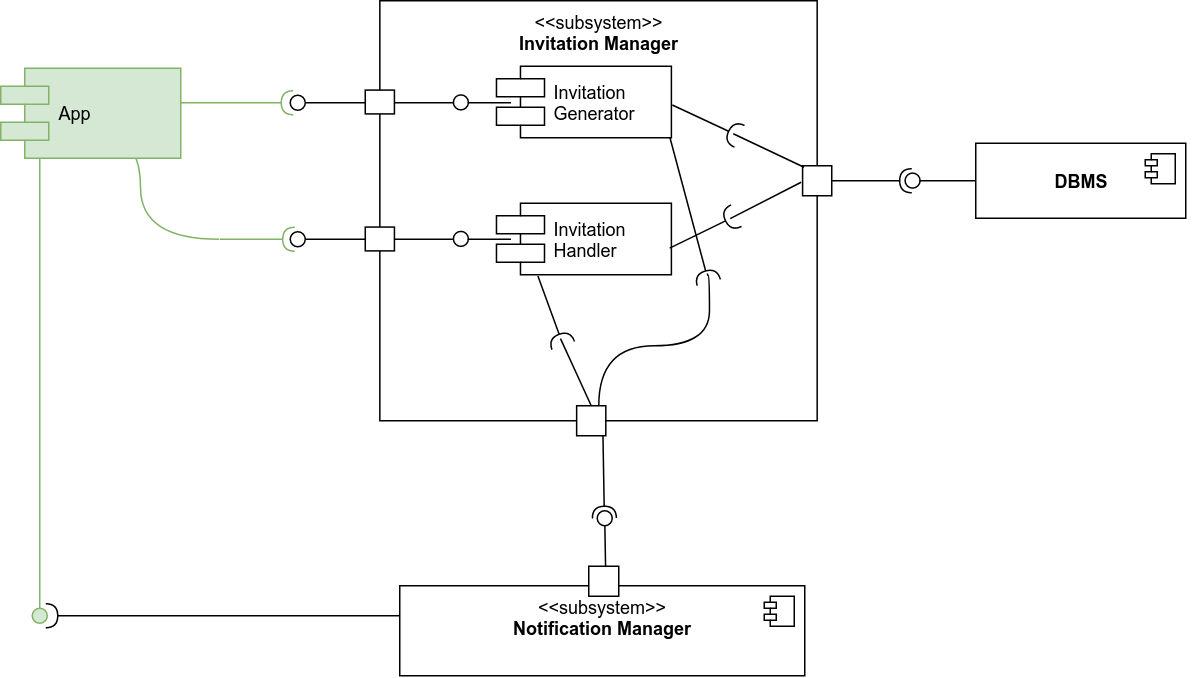
\includegraphics[width=0.9\paperwidth]{Images/CD_InvitationManager}}
			\caption{Component Diagram - Invitation Manager}
		\end{figure}
	
\subsection{Deployment view}
	% TODO
	
\subsection{Runtime view}
	\label{sect:RuntimeView}
		\begin{figure}[H]	
		\centerline{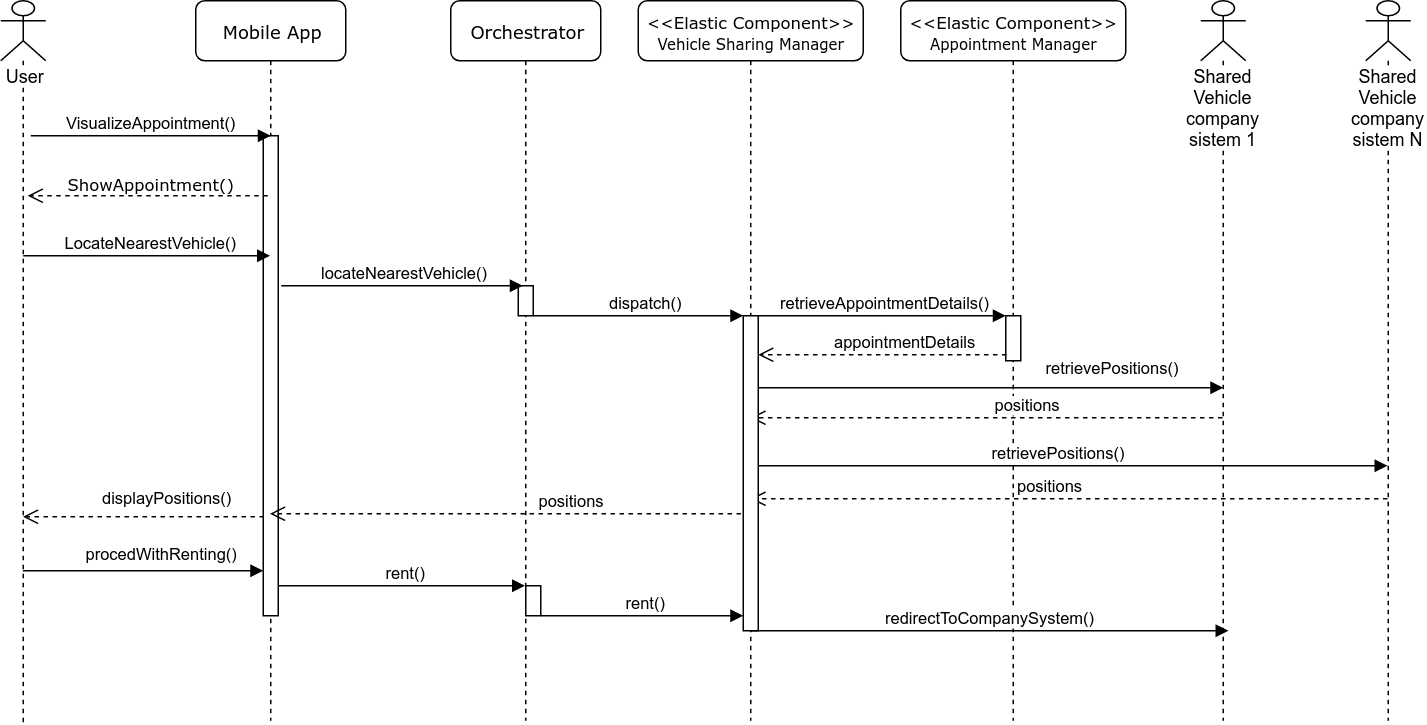
\includegraphics[width=0.9\paperwidth]{Images/LocateNearest}}
		\caption{Sequence Diagram - Locate Nearest Vehicle}
	\end{figure}
	
\subsection{Component interfaces}
	% TODO
	
\subsection{Selected architectural styles and patterns}
	% TODO
	
\subsection{Other design decisions}
	% TODO